\section{Physical properties}

When one think at the study of condensed matter, the first thing that might come to his mind is the evaluation of the properties of a material intended as its characteristics. That is indeed true to some extent, but still one question that the reader thinking at it should ask himself is: what is a matherial property? This question may seem daunting at first sight, nevertheless an incredible simple and elegant answer can be given to it in the following terms
\dfn{Physical property}
{
    A physical property is a relation between two measurable quantities.
}
\noindent
If one is not completely obscure to physics may find out that this definition fits for the description of quantities like the conductivity $\sigma$, connecting external field $\vb{E}$ and density current $\vb{J}$, or elasticity constant $K$ and so on. Therefore, this concept may seem to lead us in the right track to understand what a physical property is but to have the picture complete we shall need to define exactly what quantities can be related by such properties. We are going to classify them in \textbf{generalized forces} and \textbf{conjugate responses} which are related in the following way
\dfn{Measurable quantities}
{
    We classify the measurable quantities between generalized forces $\psi_i$ and conjugate response $\xi_i$ which are related by the following relation
    \begin{equation}
        \psi_i\dd \xi_i = \delta w,
    \end{equation}
    where $\delta w$ is the differential of work per unit volume done on the system.
}
\noindent
One can also see this definition, or distinction, on a more physical level by thinking at the generalized forces $\psi$ as stimuli that, acting on the system, generates a response $\xi$. Exactly like pressure $P$ generate a variation of volume from the system $\dd V$ that so create work $P\dd V$.

This framework also allow us to rewrite the first principle of Thermodynamics in a simpler manner since we have given a general form to the work $\delta w$ on the system. In particular, using the Einstein implicit summation formalism, we will have
\begin{equation}
    \label{eq:firstPrinciple}
    \dd u = T\dd s + \psi_i \dd \xi_i,
\end{equation}
where we can also think at the temperature as a generalized force with entropy as a response. Thus, we will write from now on $X_i$ for all the generalized forces, including temperature, and $Y_i$ for the responses having \eqref{eq:firstPrinciple} written as
\begin{equation}
    \label{eq:genFirstPrinciple}
    \dd u = X_i\dd Y_i,
\end{equation}
that will work as our \textbf{generalized first principle of thermodynamics}.

During the course we will also see how this definition of physical property also allow us to distinguish two main categories: \textbf{equilibrium properties}, that appear in a system at equilibrium such as the spring constant, and \textbf{transport properties}, that appear do to irreversible thermodynamic such has the conductivity. The main difference between the two can be thought to be the fact that in one case the material is still, in the other case average currents are present that, even if are in a stationary state, create transport of matter inside the material.

\subsection{Constitutive relation}

Once defined what a physical quantity is in general we can go and see how they look like, which is something that can be done in a first approximation making the assumption that a linear relation between forces and response are present. In this way we can assume that a general way to write down such linear relation in general is the following
\begin{equation}
    \label{eq:consRel}
    Y_i - Y_i^0 = \mathcal{K}_{ij}(X_j - X_j^0).
\end{equation}
The latter is called \textbf{constitutive relation} and effectively relates forces with responses through the tensor $\mathcal{K}$ which, therefore, contains all the physical properties. Obviously this is only a first order approximation used to evaluate the variation of the two quantities from a starting state $(\vb{X}^0, \vb{Y}^0)$, nevertheless still allow us to have a first simple way of looking at the physical properties. In fact, inside \eqref{eq:consRel} we are able to write down the entries of $\mathcal{K}$ simply using
\begin{align}
    \label{eq:defOfK}
    &\mathcal{K}_{ij} = \eval{\pderivative{Y_i}{X_j}}_{X_j=X_j^0}, &\mathcal{K} = \begin{pmatrix}
        \grad_{\vb{k}}Y_1\\
        \vdots\\
        \grad_{\vb{k}}Y_N
    \end{pmatrix}.
\end{align}
This tensor is the main object of interest in a first approximation and understanding its properties can lend us a huge help on a general ground. Luckily the definition we have given leave us a lot of space to work with and one can readily go and see easily how the following is true
\thm{Symmetry of $\mathcal{K}$}
{
    The physical property tensor $\mathcal{K}$ is a symmetric one, therefore we have
    \begin{equation}
        \mathcal{K}_{ij} = \mathcal{K}_{ji}.
    \end{equation}
}
\pf{Proof}
{
    We can consider the free energy function $g$, we know it's defined as the Legendre transform of the internal energy which in our generalized case makes us obtain the following
    \begin{align}
        &g = u - X_iY_i, &\dd g = -Y_i\dd X_i.
    \end{align}
    Since $g$ is assumed to be continuous we can use the Schwartz theorem and say that the order of the derivation doesn't matter having so that
    \begin{equation}
        \pderivative{g}{X_i}{X_j} = \pderivative{g}{X_j}{X_i},
    \end{equation}
    which, using \eqref{eq:defOfK}, turns out as
    \begin{equation}
        \mathcal{K}_{ij} = \mathcal{K}_{ji}.
    \end{equation}
}
So, before even starting to look into the actual form of $\mathcal{K}$ we already now that has certain symmetries, but it's also not so difficult to give a concrete form to this tensor by assuming the forces into play inside our system. In particular, we are going to assume that inside a solid state system the work is mainly given by the following expression
\begin{equation}
    \delta w = \vb{E}\vdot\dd\vb{D} + \vb{H}\vdot\dd\vb{B} + \vb*{\sigma}\vdot\dd\vb*{\varepsilon}.
\end{equation}
Where electric and magnetic work are presents along with the one given by the stress $\vb*{\sigma}$ and strain $\vb*{\varepsilon}$. The last two are symmetric rank two tensors that kind of generalize pressure and variation of volume. This allows us to see the various general force and responses that we need to relate, making us have a general form for the $\mathcal{K}$ tensor that look as in Fig. (\ref{fig:tensorK}). Inside that general form we can see how all the quantities are related to each others somehow,This means that the presence of an electric field not only can cause the creation of an electric polarization, generated by the on-diagonal blocks called \textbf{principal effects}, but also a magnetic one or a change in shape. These phenomenons are due to the presence of off-diagonal blocks, called \textbf{cross effects} or \textbf{interaction effects}, inside the tensor that relate the force also to non-conjugate responses. For this reason can be important to look at some of them, also to understand some important properties of these tensors. 

\begin{figure}[t]
    \centering
    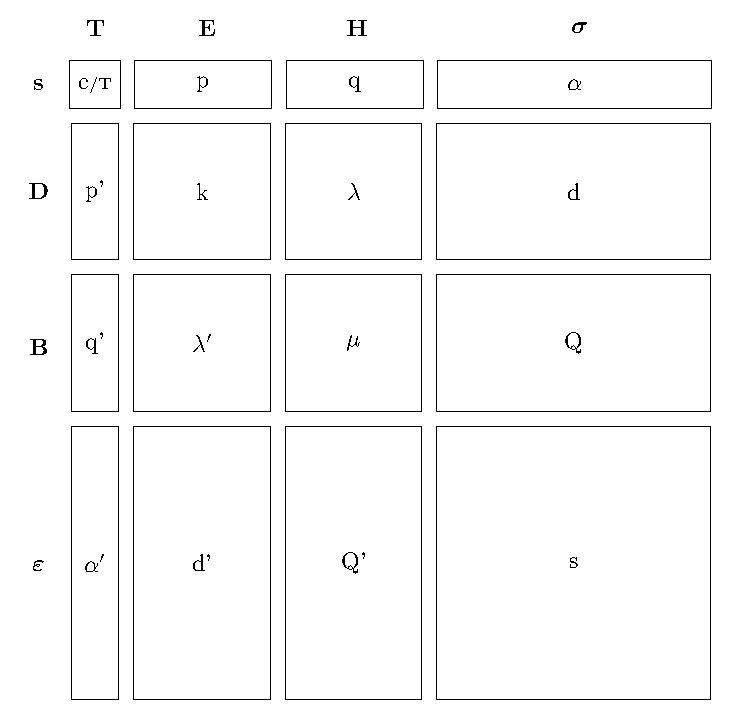
\includegraphics[width=0.6\textwidth]{Immagini/TabellaK.pdf}
    \caption{
        General form of the $\mathcal{K}$ tensor that defines the constitutive relations inside the material. The different blocks are composed by tensors of different ranks and symmetries, but the overall structure needs to be symmetric.
    }
    \label{fig:tensorK}
\end{figure}

\paragraph{c specific heat, $\vb*{T(0)}$.} Relates the temperature and the heat transmitted to the solid per unit volume at constant $\vb{E}, \vb{H}$ and $\vb*{\sigma}$. It's important to notice that is a scalar quantity, the only one inside $\mathcal{K}$, and so can be also written as $T(0)$\footnote{To identify different type of tensor we will use the notation $T(n)$, which means tensor of rank $n$.}.

\paragraph{k dielectric constant, $\vb*{T_S(2)}$.} Relates the polar vectors $\vb{E}$ and $\vb{D}$, it's known from classical electromagnetism. Also, being on the diagonal one can see that needs to be symmetric $\mathbf{k} = \mathbf{k}^\dagger$, so it's a rank two symmetric tensor, $T_S(2)$\footnote{If a tensor is symmetric the subscript $S$ is used.}, and as such has $6$ independent components. 

\paragraph{$\vb*{\mu}$ magnetic permeability, $\vb*{T_S(2)}$.} Relate two axial vectors $\vb{H}$ and $\vb{B}$, and it's also known from classical electromagnetism. The same consideration done on $\mathbf{k}$ are valid also on him being on the diagonal.

\paragraph{s elastic compliance, $\vb*{T_S(4)}$.} It generalizes Hooke's law relating stress with deformation which are rank two tensors, making it a rank four that write down the relation of the two as
\begin{equation}
    \varepsilon_{ij} = s_{ijkl} \sigma_{kl}.
\end{equation}
Also, in this case the tensor is symmetric since $\vb*{\varepsilon}$ and $\vb*{\sigma}$ are having so $s_{ijkl} = s_{klij}$, this make so that the total number of independent variables in the tensor are $21$. The inverse of this tensor, $\mathbf{c}$, is called \textbf{elastic stiffness}.

\paragraph{p electrocaloric effect, $\vb*{T(1)}$.} Describes how an external electric field can generate heat inside a material changing entropy and so temperature. Since $\mathcal{K}$ is symmetric we need to have $\vb{p} = \vb{p}'$.

\paragraph{p' pyroelectric effect, $\vb*{T(1)}$.} Describe the electric polarization generated by variation of the material's temperature.

\paragraph{q magnetocaloric effect, $\vb*{T^{ax}(1)}$.} Describes the variation of temperature generated by an external magnetic field. Also, since we will have that $T\vb{q} = \vb{H}$ we will need $\vb{q}$ to be a pseudo-vector, therefore the tensor is called an axial one\footnote{We will describe axial tensor with the upscript $ax$, mathematically are objects that are not invariant to parity transformations.}.

\paragraph{q' pyromagnetic effect. $\vb*{T^{ax}(1)}$.} Describe Magnetization induced by temperature changes, and from symmetry we once again have $\vb{q} = \vb{q}'$.

\subsection{Symmetry is important}

In the simple description of the constitutive relation that we give previously inside a simple linear approximation was already simple to grasp how the symmetry of $\mathcal{K}$ helped us in the understanding of some phenomena. For example, we found out that if the $\vb{p}$ entries are non-zero we have electrocaloric effect, and with it also $\vb{p}'$ needs to be non-zero having so also the pyroelectric effect. Therefore, only by simple symmetry we see how several effects are related to each others, but we can go deeper and the way to do that rely on a simple but incredibly clever princple thought by Nuemann that assume the following.
\thm{Nuemann principle}
{
    The symmetry of any physical property of a material can not be lower than the symmetry of its atomic-level structure.
}
\pf{Proof}
{
    This is not really a proof of the principle, it's more an explanation of the logic on which is based. The idea is that if I make a rotation to the system and the atomic structure doesn't change, due to symmetry, therefore I have the exact same material and interactions. This implies that, if the latter was true, also all the properties of the material should not have changed. Mathematically, this translates to the invariance of the mathematical object to the action of the group elements inside the point group of the crystal.
}

\noindent
To understand to what extent the utility of this principle we can look at some cases of application to some quantities. For example, let's imagine having a crystal with inversion as a symmetry and see what happens to rank ones tensors. Therefore, let's assume to have the tensor $\vb{p} = (p_x, p_y, p_z)$ if the system have inversion symmetry the following needs to be true
\begin{equation}
    \begin{pmatrix}
        p_x\\
        p_y\\
        p_z
    \end{pmatrix} = \begin{pmatrix}
        -1 & 0 & 0\\
        0  &-1 & 0\\
        0  & 0 &-1
    \end{pmatrix}
    \begin{pmatrix}
        p_x\\
        p_y\\
        p_z
    \end{pmatrix} = \begin{pmatrix}
        -p_x\\
        -p_y\\
        -p_z
    \end{pmatrix}.
\end{equation}
This clearly makes so that the only possible solution to the equation to make the vector invariant is $\vb{p} = \vb{0}$, meaning that in a crystal with inversion symmetry no $T(1)$, or $T(0)$, properties can be present. This is already a powerful result that let us know which materials can possibly show some properties. Another interesting thing to see is looking at the presence of rotational symmetries which allow us to have the following result
\cor{}
{
    If a rotation symmetry is inside the point group of the crystal the $T(1)$ properties can only have non-zero entries only in the direction of the axis of rotation called \textbf{polar direction}.
}
\pf{Proof}
{
    Let the group $C_n$ be a subgroup of the point group, and we assume that the rotation axes is in $z$ direction, so that if we need to make a $T(1)$ invariant respect to the rotation we will require the following
    \begin{equation}
        \begin{pmatrix}
            p_x\\
            p_y\\
            p_z
        \end{pmatrix} = \begin{pmatrix}
            \cos(2\pi/n) & \sin(2\pi/n) & 0\\
            -\sin(2\pi/n)  &\cos(2\pi/n) & 0\\
            0  & 0 &1
        \end{pmatrix}
        \begin{pmatrix}
            p_x\\
            p_y\\
            p_z
        \end{pmatrix} = \begin{pmatrix}
            \cos(2\pi/n)p_x + \sin(2\pi/n)p_y\\
            \cos(2\pi/n)p_y - \sin(2\pi/n)p_x\\
            p_z
        \end{pmatrix}.
    \end{equation}
    To solve the equation it's easy to see how $p_x = p_y = 0$ while only the component in the polar direction can be non-zero.
}

The same principle can be applied to other rank tensors, and becomes really important for rank two ones $\mathbf{T}$ where the requirement for respecting a ceratain symmetry $\mathbf{R}$ simply becomes
\begin{equation}
    \mathbf{T} = \mathbf{R}\mathbf{T}\mathbf{R}^{-1}.
\end{equation}
Applied to general matrix using specific high symmetry point groups allows for a huge simplification of the independent components inside the tensor. The simplest, and probably most important, case is the one of a crystal with cubic symmetry, which bring the possibilities to one
\cor{}
{
    Inside a cubic crystal all the $T(2)$ properties are isotropic, therefore have only one independent component and can be written as $\mathbf{A} = A\mathbf{1}$.
}
\noindent
I'm not going to do the computations, but in reality are really easy since you only need to impose two \SI{90}{\degree} rotations on different axis. 

\nt
{
    This particular case forms also a counterexample to prove how the Neumann principle doesn't work backwards, meaning that it's possible how a physical property shows greater symmetry than the crystal itself. In fact, in this case the $T(2)$ becomes a scalar which is invariant under any type of rotational symmetry, while the cubic crystal has only $C_4$ at best.
}

\subsection{Time symmetry}

One last type of symmetry was left out by the latter discussion, in fact inside magnetic crystals the orientation of the magnetic moment may add another degree of symmetry. If we assume that all magnetic phenomena can be associated to the presence of moving charge, and so currents, then also the \textbf{time reversal symmetry} $\vb*{\Theta}$ becomes important. In particular one can call \textbf{i-tensors} the ones that are invariant under $\vb*{\Theta}$ and \textbf{c-tensors} the others we will have that the magnetic field is inside the latter, having
\begin{equation}
    \mathbf{H}(-t) = -\mathbf{H}(t).
\end{equation} 
The same thing can be applied to the $\mathcal{K}$ matrix and add also time-symmetry to the Nuemann principle. In particular the physical quantity needs to be compatible with the properties of the quantities that relates, for example let's consider $\mathbf{X}$ and $\mathbf{Y}$ both i or c-tensors we can write
\begin{equation}
    \vb*{\Theta}\mathbf{Y} = \pm\mathbf{Y} = \pm\mathcal{K}\mathbf{X} = \vb*{\Theta}\mathcal{K}\mathbf{X}.
\end{equation}
Which simply translates to no further restrictions to the properties of the physical quantities. Instead, if we have that $\mathbf{X}$ and $\mathbf{Y}$ are opposite time reversal tensors, in that case the relation between the two becomes
\begin{equation}
    \vb*{\Theta}\mathbf{Y} = -\mathbf{Y} = -\mathcal{K}\mathbf{X} = \vb*{\Theta}\mathcal{K}\mathbf{X}.
\end{equation}
This leads to the fact that $\vb*{\Theta}\mathcal{K} = -\mathcal{K}$ giving rise an increase of the symmetry inside the tensor. Also, if we assume that $\mathcal{K}$ is a c-tensor in the specific case we are looking we obtain $\mathcal{K} = -\mathcal{K}$ saying to us that the tensor needs to be identically zero.

The properties that relate different time-symmetry tensors are, therefore, special and takes the name of \textbf{special magnetic properties}. Some examples of such properties are the magnetocaloric effect $p_i$, magnetoelectric polarization $\lambda_{ij}$ and piezomagnetism $Q_{ijkl}$.